\documentclass[11pt]{article}

\usepackage[doublespacing]{setspace}
\usepackage{amsfonts,amsmath,amssymb, amsthm, color, graphicx,graphics,verbatim}
\usepackage{apacite}
\usepackage[left=2cm,textheight=9in,right=2cm]{geometry}
\usepackage{bm}
\usepackage{url}
\usepackage[
singlelinecheck=false % <-- important
]{caption}
\usepackage{multirow}
\usepackage{makecell}
\usepackage{natbib}
%\usepackage{harvard}\\
\usepackage{hyperref}
\usepackage{epstopdf}
\usepackage{pdflscape}
\usepackage{longtable}
\usepackage{caption}
\usepackage{subcaption}
\usepackage{tablefootnote}
\usepackage{dcolumn,booktabs}
\usepackage{bm}
\usepackage{float}
\usepackage{titlesec}
\graphicspath{{./images/}}
\titleformat{\section}{\bfseries}{\thesection.}{1em}{}
\titlespacing{\section}{0pt}{12pt}{6pt}
\titleformat{\subsection}{\bfseries}{\thesubsection.}{1em}{}
\titlespacing{\subsection}{0pt}{12pt}{6pt}
\setcounter{secnumdepth}{4}

\titleformat{\paragraph}
{\normalfont\normalsize\bfseries}{\theparagraph}{1em}{}
\titlespacing*{\paragraph}
{0pt}{3.25ex plus 1ex minus .2ex}{1.5ex plus .2ex}
\newcolumntype{d}[1]{D..{#1}} % define a "decimal" column type
\newcommand\mc[1]{\multicolumn{1}{c}{#1}} % a handy shortcut macro
%\setlength\parindent{0pt} % just for this example
\begin{document}
	\newpage
	\begin{center}
		\textbf{Problem Set 1 Response} 
		
		Campbell Clarkson
	\end{center}
	
	\section{Dataset and Figures}\label{section1}
	
	\noindent I am introducing a dataset I am working on with a student from the College of Computing. We are building a machine learning project for song recognition, so the figures here use acoustic data points from 2000 popular spotify songs.
	
	\begin{center}
	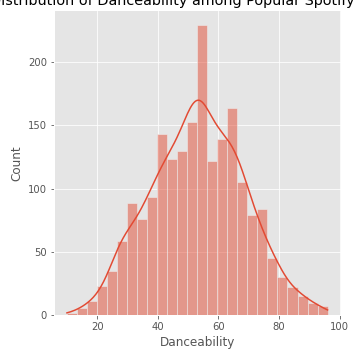
\includegraphics[scale=1]{dance_hist}\label{dist}
	\end{center}
	
	In figure \ref{dist}, this examines the distribution of ''danceability'' among the dataset, where it is clear it follows a normal distribution. This may be useful when we train our dataset to recognize a song with danceability as a factor. Does danceability have any bearing on popularity, though? 
	
	\begin{center}
		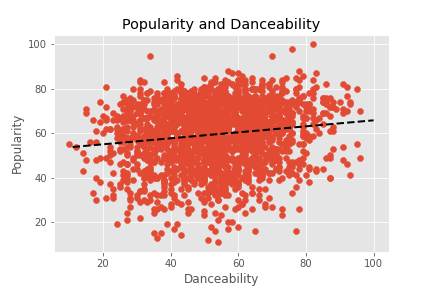
\includegraphics[scale=1]{dance_pop_scatter}\label{scat_dance}
	\end{center}

	From this figure \ref{scat_dance}, it's apparent that the more ''danceable'' a song is, according to Spotify's metrics, then the more popular it tends to be. Let's consider some other metrics then, which may be useful. What happens when we look at both song tempo and the valence (in other words, how happy the song sounds) on its popularity.
	
	\begin{center}
		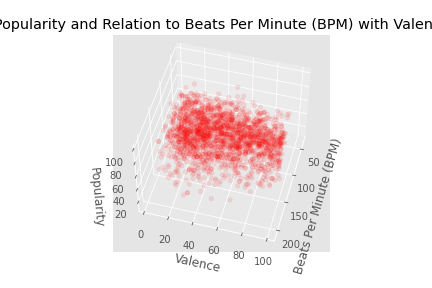
\includegraphics[scale=1]{3dplot}\label{3d}
	\end{center}
	
	It's unclear whether tempo and valence together have a specific bearing on popularity when examining this plot. However, examining this data with a proper model could prove useful to see which qualities are most important for a song's popularity or the optimal song to maximize popularity.
	
\end{document}
